\usepackage{lmodern}
\usepackage{amssymb,amsmath,mathtools,amsthm}
\usepackage[T1]{fontenc}
\usepackage[utf8]{inputenc}
\usepackage{textcomp} % provide euro and other symbols

\usepackage{pgfpages}

\usepackage{multirow}
\usepackage{csvsimple}
\usepackage{siunitx}

% prevent slide breaks in the middle of a paragraph
\widowpenalties 1 10000
\raggedbottom


% Use upquote if available, for straight quotes in verbatim environments
\usepackage{upquote}
\usepackage[]{microtype}
\UseMicrotypeSet[protrusion]{basicmath} % disable protrusion for tt fonts

\usepackage{xcolor}
\usepackage{xurl} % add URL line breaks if available
\usepackage{bookmark}
\usepackage{hyperref}
\hypersetup{
  colorlinks = true,
  linkcolor  = Maroon,
  filecolor  = Maroon,
  citecolor  = Blue,
  urlcolor   = Blue
}

% tikz and pgfplots stuff
\usepackage{tikz}
\usetikzlibrary{arrows,shapes,positioning,intersections}
\usepackage{pgfplots}
\usepgfplotslibrary{external,colormaps}
\pgfplotsset{width=7cm,compat=1.11}
%\tikzexternalize

\newif\ifbibliography
\setlength{\emergencystretch}{3em} % prevent overfull lines
\setcounter{secnumdepth}{-\maxdimen} % remove section numbering

%\usepackage{subfig}
\usepackage{subcaption}
\usepackage{algorithm,algpseudocode}
\usepackage{booktabs}


% biblatex
\usepackage[citestyle=authoryear]{biblatex}
\addbibresource{references.bib}

\AtBeginPart{\frame{\partpage}}
\AtBeginSection{\ifbibliography\else\frame{\sectionpage}\fi}
\AtBeginSubsection{\frame{\subsectionpage}}

\usetheme{boxes}
\usecolortheme{beaver}
\usefonttheme{professionalfonts}
\usefonttheme{structurebold}
\setbeamertemplate{footline}[frame number]
\setbeamertemplate{caption}[numbered]
\setbeamertemplate{caption label separator}{: }
\setbeamercolor{caption name}{fg=normal text.fg}
\setbeamertemplate{itemize item}{\(\bullet\)}
\setbeamertemplate{itemize subitem}{\(\circ\)}
\setbeamertemplate{itemize subsubitem}{\textendash}
\setbeamerfont{frametitle}{size=\large}
\setbeamerfont{framesubtitle}{size=\small}
% \setbeamertemplate{headline}{\vskip4ex}
\beamertemplatenavigationsymbolsempty

% operators
\DeclareMathOperator*{\argmax}{arg\,max}
\DeclareMathOperator*{\argmin}{arg\,min}
\DeclareMathOperator{\sign}{sign}
\DeclareMathOperator{\E}{E}
\DeclareMathOperator{\var}{Var}

% macros
\newcommand{\pkg}[1]{\textsf{#1}}
\renewcommand{\vec}[1]{\bm{#1}}
\newcommand{\mat}[1]{\bm{#1}}
\newcommand{\du}{\mathrm{d}}



% title block
\title{The Hessian Screening Rule and Adaptive Paths for the Lasso}
\subtitle{Wroclaw Technical University Seminar}
\author{Johan Larsson}
\institute{Department of Statistics, Lund University}
\date{\today}
\titlegraphic{\includegraphics{figures/logo.pdf}}

\begin{document}

\frame[noframenumbering,plain]{\titlepage}

\begin{frame}{Overview}
  \tableofcontents[hideallsubsections]
\end{frame}

\section{Preliminaries}

\begin{frame}{The Lasso}
  A type of penalized regression, represented by the following
  convex optimization problem:
  \[
    \operatorname*{minimize}_{\beta \in \mathbb{R}^p}
    \left\{
      f(\beta) + \lambda \lVert \beta \rVert_1.
    \right\}
  \]
  where \(f(\beta)\) is smooth and convex. \medskip

  \begin{columns}[T]
    \begin{column}{0.45\linewidth}
      \(f(\beta) = \frac 1 2 \lVert y - X\beta\rVert_2^2\)
      leads to the ordinary lasso \medskip

      \(\lambda\) is a hyper-parameter that controls the level of
      \alert{penalization}. \medskip

      \(\hat\beta(\lambda)\) is the solution to this problem for a given
      \(\lambda.\)

    \end{column}
    \begin{column}{0.45\linewidth}
      \begin{figure}
        \centering
        \pgfplotsset{width=6cm,height=6cm}
        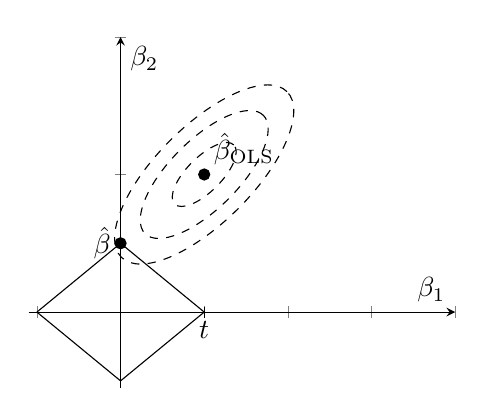
\begin{tikzpicture}
\begin{axis}[
    xlabel = \(\beta_1\),
    ylabel = \(\beta_2\),
    ymin = -1.1,
    ymax = 4,
    xmin = -1.1,
    xmax = 4,
    axis lines = center,
    yticklabels={,,},
    xticklabels={,,}
]
\draw[dashed, rotate around={45:(1,2)}] (1,2) ellipse (0.5 and 0.25);
\draw[dashed, rotate around={45:(1,2)}] (1,2) ellipse (1 and 0.5);
\draw[dashed, rotate around={45:(1,2)}] (1,2) ellipse (1.4 and 0.7);

\addplot[]
    coordinates {
    	(-1,0)
    	(0,1)
    	(1,0)
    	(0,-1)
    	(-1,0)
    };
    
\addplot [only marks, mark=*] coordinates {(1,2)};
\node [above right,black] at (1,2) {\(\hat\beta_\text{OLS}\)};

\addplot [only marks, mark=*] coordinates { (0,1) };
\node [left] at (0,1) {$\hat\beta$};

\addplot [only marks, mark = |] coordinates { (1, 0) };
\node [below] at (1,0) {\(t\)};
\end{axis}
\end{tikzpicture}
      \end{figure}
    \end{column}
  \end{columns}
\end{frame}

\begin{frame}{The Lasso Path}
  Solving the lasso for \(\lambda \in [0, \lambda_\text{max})\), with
  \[\lambda_\text{max} \coloneqq \max \big\{ \lambda \in \mathbb{R}^+ \mid
  \hat\beta(\lambda) = 0\big\},\]
  traces the set of all solutions for the lasso:
  the (exact) lasso path. \medskip

  \pause

  \begin{columns}[T, onlytextwidth]
    \begin{column}{0.5\linewidth}
      \begin{itemize}
        \item Piece-wise linear with breaks wherever the
          active set changes \medskip
        \item The size of the active set cannot exceed \(n\), the number of
          observations.
      \end{itemize}
    \end{column} 
    \begin{column}{0.5\linewidth}
      \begin{figure}
        \includegraphics{figures/lasso-path}
        \caption{The lasso path for an example of the standard lasso}
      \end{figure}
    \end{column}
  \end{columns}

\end{frame}

\begin{frame}{Picking \(\lambda\)}

  \begin{block}{The Problem}
    Typically don't know the optimal value for
    \(\lambda\). To tackle this, we use cross-validation to tune for
      \(\lambda\).
  \end{block}

  \pause

  \begin{block}{Grid Search}
    For \(p \gg n\), the standard procedure is to create a
    grid of \(\lambda\)s and solve the lasso numerically.
  \end{block}

  \medskip

  \pause

  But this is computationally demanding when \(p\) is large.
  
\end{frame}

\subsection{Screening Rules}

\begin{frame}{Predictor Screening Rules}
  \begin{block}{Motivation}
    Many solutions along the regularization path are \alert{sparse}, 
    especially if \(p \gg n\).
  \end{block}

  \pause

  \begin{block}{Basic Idea}
    Say that we are at step \(k\) on the lasso path and are about to solve for
    step \(k + 1\). \medskip

    Intuitively, information at \(k\) should tell us something
    about which predictors are going to be non-zero at step \(k + 1\). \medskip

    Idea is to use this information to \alert{discard} a subset of the
    predictors and fit the model to a smaller set of predictors---the screened
    set.
  \end{block}
\end{frame}

\begin{frame}{Types of Screening Rules}
  \begin{block}{Safe Rules}
    Certifies that discarded predictors are inactive at the optimum.
  \end{block}
  \pause
  \begin{block}{Heuristic (Un-Safe) Rules}
    No guarantees! Result in \alert{violations}: discarding predictors that
    actually will be active. \medskip

    Need post-optimization checks of optimality
    conditions. \medskip

    Checking the optimality conditions can be costly.
  \end{block}
\end{frame}

\begin{frame}{Optimality Conditions}
  \(\beta\) is a solution to the lasso problem if it satisfies the stationarity
  criterion
  \[
    \boldsymbol{0} \in \nabla f(\beta) + \lambda \partial
  \]
  where \(\partial\) is the subdifferential of \(\lVert \beta \rVert_1\),
  defined as
  \[
    \partial_j \in
    \begin{cases}
      \{\sign(\beta_j)\} & \text{if } \beta_j \neq 0, \\
      [-1,1]             & \text{otherwise.}
    \end{cases}
  \]
  \pause
  This means that
  \[
    |\nabla f(\beta)_j| < \lambda \implies \hat\beta_j = 0.
  \]
  Of course, we don't know \(\nabla f(\beta)\) prior to solving the problem.

  % TODO: insert subdifferential plot
\end{frame}

\begin{frame}{The Gradient Perspective of the Path}
  \begin{figure}
    \input{figures/lasso-path-gradient.tikz}
    \caption{The gradient vector along the lasso path}
  \end{figure}
\end{frame}

\begin{frame}{Screening Rules as a Gradient Estimate}
  Let \(c(\lambda) \coloneqq -\nabla f(\beta(\lambda))\)
  be the so-called \alert{correlation} vector.

  \medskip

  \(\boldsymbol{0} \in \nabla f(\beta)
  + \lambda \partial\) suggests a simple template for a screening rule:
  \begin{enumerate}
    \item replace \(-\nabla f(\beta)\) with an estimate \(\tilde c\)
    \item rule: if \(|\tilde c_j| < \lambda\), discard predictor \(j\).
  \end{enumerate}
  
  \medskip
  
  If \(\tilde c\) is accurate and not too conservative, we
  have a useful rule.
\end{frame}

\begin{frame}{The Strong Rule}
  The Strong Rule gradient estimate is
  \[
    \tilde c^S(\lambda_{k+1}) =
    \underbrace{c(\lambda_k)}_\text{previous gradient} +
    \underbrace{(\lambda_k - \lambda_{k+1})\sign(c(\lambda_k))}_\text{unit
      slope
      bound}.
  \]
  \begin{columns}[T]
    \begin{column}{0.45\linewidth}
      \alert{simple idea}\\
      assume that the slope of the gradient is bounded by one (the
      unit slope bound)~\parencite{tibshirani2012}
    \end{column}
    \begin{column}{0.45\linewidth}
        \centering
        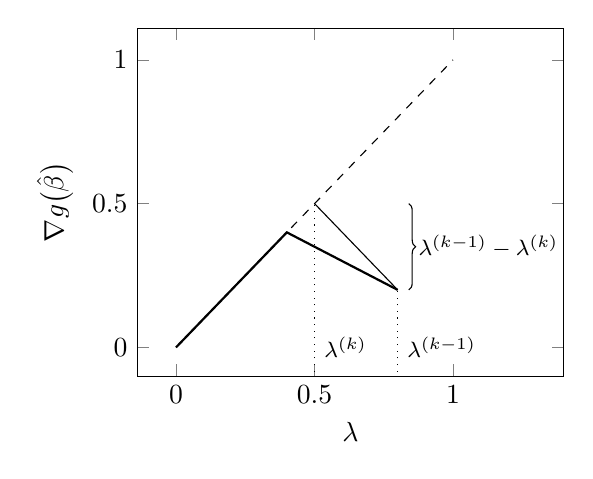
\begin{tikzpicture}
\begin{axis}[
    ylabel = \(\nabla g\big(\hat\beta\big)\),
    xlabel = \(\lambda\),
    xmax = 1.4,
    ymin = -0.1,
    width = 7cm,
    height = 6cm
]
\addplot[style = dashed]
    coordinates {
        (0,0)
        (1,1)
    };
\addplot[]
    coordinates {
        (0.8,0.2)
        (0.5,0.5)
    };
\addplot[thick]
    coordinates {
        (0.8,0.2)
        (0.4,0.4)
        (0,0)
    };
\draw [decorate,decoration={brace},xshift=4pt]
(0.8,0.5) -- (0.8,0.2)node [right,black,midway] {\footnotesize
$\lambda^{(k-1)}-\lambda^{(k)}$};

\addplot[style=dotted]
    coordinates {
        (0.5,-0.2)
        (0.5,0.5)
    };
\addplot[style=dotted]
    coordinates {
        (0.8,-0.2)
        (0.8,0.2)
    };
\node [right] at (0.5,0) {\footnotesize$\lambda^{(k)}$};
\node [right] at (0.8,0) {\footnotesize$\lambda^{(k-1)}$};
\end{axis}
\end{tikzpicture}
        % \caption{The unit slope bound}
    \end{column}
  \end{columns}
\end{frame}

\begin{frame}{The Working Set Algorithm}
  The Strong Rule is conservative when predictors are correlated. \medskip

  A better alternative is to use the predictors that have
  \alert{ever been active} as a screened set and then
  \begin{enumerate}
    \item fit the lasso on the predictors in the screened set,
    \item check the optimality conditions in the strong set, and then
    \item check the optimality conditions for all predictors.
  \end{enumerate}
  Whenever we encounter violations (in step 2 or 3), go back to step 1 and
  repeat.
\end{frame}

\section{The Hessian Screening Rule}

\begin{frame}{The Ordinary Lasso}
  We now focus on the ordinary lasso, \(\ell_1\)-regularized least
  squares:
  \[
    f(\beta) = \frac 1 2 \lVert y - X\beta \rVert_2^2
  \]
  and
  \[
    \nabla f(\beta) = X^T(X\beta - y).
  \]
  \pause
  It turns out that we can express the solution as a function of
  \(\lambda\):
  \begin{equation*}
    \label{eq:solution}
    \hat\beta(\lambda) = \big({X_\mathcal{A}}^TX_\mathcal{A}\big)^{-1}
    \big({X_\mathcal{A}}^Ty - \lambda \sign(\hat\beta_\mathcal{A})\big).
  \end{equation*}
  \pause
  This expression holds for an interval \([\lambda_k,\lambda_{k+1}]\) in which
  no changes occur in the active set, which means we can retrieve any solution
  in this range via
  \begin{equation*}
    \hat\beta(\lambda_{k+1})_\mathcal{A} =
    \hat\beta(\lambda_k)_\mathcal{A} -
    (\lambda_k - \lambda_{k+1})\big({X_\mathcal{A}}^TX_\mathcal{A}\big)^{-1}
    \sign\big(\hat\beta(\lambda_k)_\mathcal{A}\big).
  \end{equation*}
\end{frame}

\begin{frame}{The Hessian Screening Rule}
  Take this expression and stick it into the gradient at step \(k +
  1\):
  \begin{equation*}
    \begin{aligned}
      \tilde c^H(\lambda_{k+1})
       & = -\nabla f\big(\hat\beta(\lambda_{k+1})_\mathcal{A}\big)       \\
       & = c(\lambda_k) + (\lambda_{k+1} - \lambda_k)X^T {X_\mathcal{A}}
      \big({X_\mathcal{A}}^T{X_\mathcal{A}}\big)^{-1}
      \sign\big(\hat\beta(\lambda_k)_\mathcal{A}\big),
    \end{aligned}
  \end{equation*}
  which is the basic form of our screening rule: \alert{The Hessian Screening
    Rule}. \medskip

  Note that this is an exact expression for the correlation vector (negative
  gradient) at step \(k+1\) if the activate set has remained unchanged.\medskip

  The Hessian Screening Rule is a heuristic (un-safe) rule: it may result in
  violations.
\end{frame}

\begin{frame}{The Hessian and Strong Screening Rules}
  \begin{figure}
    \input{figures/estimate-comp.tikz}
    \caption{Conceptual comparison of screening rules}
  \end{figure}
\end{frame}

\begin{frame}{Tweaks}
  \begin{block}{Avoiding Expensive Inner Products}
    The expression
    \begin{equation*}
      \hat c^H(\lambda_{k+1})
      = c(\lambda_k) + (\lambda_{k+1} - \lambda_k)X^T {X_\mathcal{A}}
      \big({X_\mathcal{A}}^T{X_\mathcal{A}}\big)^{-1}
      \sign\big(\hat\beta(\lambda_k)_\mathcal{A}\big),
    \end{equation*}
    involves an expensive inner product with the full design matrix.
    \medskip

    Instead, we replace \(X\) with the columns indexed by the strong rule.
  \end{block}

  \pause

  \begin{block}{Upwards Shift}
    We need some upwards bias on the estimate or else risk excessive numbers of
    violations. We add a fraction \(\gamma\) of the unit bound\footnote{We've
      set \(\gamma = 0.01\) in our simulations, which has worked very well.}.
  \end{block}

\end{frame}

\begin{frame}{Warm Starts}
  The availability of the Hessian inverse enables a better warm start:
  \[
    \hat\beta(\lambda_{k+1})_\mathcal{A} \coloneqq
    \hat\beta(\lambda_k)_\mathcal{A} +
    (\lambda_k - \lambda_{k+1}) \big({X_\mathcal{A}}^T{X_\mathcal{A}}\big)^{-1}
    \sign\big(\hat\beta(\lambda_k)_\mathcal{A}\big)
  \]
  \pause
  \begin{figure}
    \centering
    \includegraphics{figures/hessian-warm-starts}
    \caption{Number of passes of coordinate descent for two datasets
      using either Hessian warm
      starts or standard warm starts.}
  \end{figure}

\end{frame}

\begin{frame}{Updating the Hessian}
  Computing the Hessian and its inverse naively is expensive:
  \(\mathcal{O}(|\mathcal{A}|^3 + |\mathcal{A}|^2n)\)

  \medskip

  Fortunately, we can sweep columns of the Hessian and inverse in our out,
  yielding complexity
  \begin{itemize}
    \item \(\mathcal{O}(|\mathcal{D}|^2n + n|\mathcal{D}||\mathcal{E}| +
          |\mathcal{D}^2||\mathcal{E}| + |\mathcal{D}|^3)\) when
          augmenting the Hessian and
    \item \(\mathcal{O}(|\mathcal{C}|^3 + |\mathcal{C}|^2|\mathcal{E}| +
          |\mathcal{C}||\mathcal{E}|^2)\) when reducing it,
  \end{itemize}
  where 
  \begin{itemize}
    \item \(\mathcal{C} = \mathcal{A}_{k-1} \setminus \mathcal{A}_k\) 
      (to-be deactivated)
    \item \(\mathcal{D} = \mathcal{A}_k \setminus \mathcal{A}_{k-1}\)
      (to-be activated)
    \item \(\mathcal{E} = \mathcal{A}_k \cap \mathcal{A}_{k-1}\)
      (still activate)
  \end{itemize}
\end{frame}

\begin{frame}{General Loss Functions}

  The rule can be extended to many other loss functions in the family of
  generalized linear models.

  \medskip

  Omit details here, but note that
  \begin{itemize}
    \item the gradient estimate now involves a matrix of weights---for logistic
      regression a diagonal matrix,
    \item the lasso path is no longer piece-wise linear, and
    \item updating the Hessian is no longer cheap.
  \end{itemize}
\end{frame}

\subsection{Results}

\begin{frame}{Setup}
  \begin{itemize}
    \item Rows of the predictor matrix i.i.d. from
          \(\mathcal{N}(0,\Sigma)\)
    \item Response generated from \(\mathcal{N}(X\beta,\sigma^2 I)\)
          with
          \(\sigma^2 = \beta^T\Sigma \beta/\text{SNR}\)
    \item \(s\) non-zero coefficients, equally spaced throughout the
        coefficient vector
  \end{itemize}

  \begin{block}{Scenario 1 (Low-Dimensional)}
    \(n = 10\,000\), \(p = 100\), \(s = 5\), and \(\text{SNR} = 1\)
  \end{block}

  \begin{block}{Scenario 2 (High-Dimensional)}
    \(n = 400\), \(p = 40\,000\), \(s = 20\), and \(\text{SNR} = 2\)
  \end{block}

  \medskip

  Code is located at

  \href{https://github.com/jolars/HessianScreening}{\nolinkurl{github.com/jolars/HessianScreening}}
\end{frame}

\begin{frame}{Simulated Data}

  \begin{figure}
    \centering
    \includegraphics{figures/simulateddata-timings}
    \caption{Time to fit a full regularization path for
      \(\ell_1\)-regularized least-squares and logistic regression to
      a design with \(n\) observations, \(p\) predictors, and pairwise
      correlation between predictors of \(\rho\). Time is relative to the
      minimal value for each group.}
  \end{figure}

\end{frame}

\begin{frame}{Real Data: Least-Squares Regression}
  \begin{table}
    \caption{Time to fit a full regularization path of \(\ell_1\)-regularized
      least-squares regression to real data sets.}
    \csvreader[
      tabular={
          l
          S[table-format=6.0,round-mode=off]
          S[table-format=7.0,round-mode=off]
          S[table-format=0.4,round-precision=2]
          S[table-format=5.2]
          S[table-format=3.3]
          S[table-format=3.2]
          S[table-format=3.2]
        },
      before reading=\notsotiny\centering\sisetup{round-mode=figures,
        round-precision=3},
      table head=\toprule & & & & \multicolumn{4}{c}{Time (s)} \\
      \cmidrule(lr){5-8} Dataset & {\(n\)} & {\(p\)} & {Density} & {Gap Safe}
      &
      {Hessian} & {Working} & {EDPP} \\\midrule,
      table foot=\bottomrule
    ]%
    {tables/realdata-timings-gaussian.csv}%
    {dataset=\dataset, n=\n, p=\p, density=\density, GapSafe=\gapsafe,
      Hessian=\hessian, Working=\working,
      EDPP=\edpp}%
    {\dataset & \n & \p & \density & \gapsafe & \hessian & \working & \edpp}
  \end{table}
\end{frame}

\begin{frame}{Real Data: Logistic Regression}

  \begin{table}
    \caption{Time to fit a full regularization path of \(\ell_1\)-regularized
      logistic regression to real data sets.}
    \csvreader[
      tabular={
          l
          S[table-format=5.0,round-mode=off]
          S[table-format=7.0,round-mode=off]
          S[table-format=1.5,scientific-notation=fixed]
          S[table-format=5.2]
          S[table-format=4.2]
          S[table-format=4.2]
        },
      before reading=\scriptsize\centering\sisetup{round-mode=figures,
        round-precision=2},
      table head=\toprule & & & & \multicolumn{3}{c}{Time (s)} \\
      \cmidrule(lr){5-7} Dataset & {\(n\)} & {\(p\)} & {Density} & {Gap Safe}
      &
      {Hessian} & {Working}\\\midrule,
      table foot=\bottomrule
    ]%
    {tables/realdata-timings-binomial.csv}%
    {dataset=\dataset, n=\n, p=\p, density=\density, GapSafe=\gapsafe,
      Hessian=\hessian, Working=\working}%
    {\dataset & \n & \p & \density & \gapsafe & \hessian & \working}
  \end{table}

\end{frame}

\begin{frame}{Discussion}
  \begin{itemize}
    \item simple, intuitive, idea
    \item performs well in our examples
    \item handles the highly-correlated case very well
    \item works for arbitrary loss functions that are twice differentiable
    \item works for other penalty functions too (SLOPE, lasso variations)
    \item a paper is submitted and under review, but a pre-print is
      available~\parencite{larsson2021}.
  \end{itemize}
\end{frame}

\section{Adaptive Lasso Path (Work in Progress)}

\begin{frame}{Standard Grid Setup}
  The dominating choice for constructing the lasso path in the high-dimensional
  regime is to setup a log-spaced grid from \(\lambda_\text{min}\) to
  \(\lambda_\text{max}\) where
  \[
    \lambda_\text{min} =\lambda_\text{max} \times
    \begin{cases}
      10^{-2} & \text{if } p > n  \\
      10^{-4} & \text{otherwise.}
    \end{cases}
  \]
  Why this particular choice? We don't know.

  \begin{block}{Why Not Use LARS?}
    Homotopy methods scale poorly with \(p\), in the worst case requiring
    \((3^p
    + 1)/2\) steps
  \end{block}
\end{frame}

\begin{frame}{The Problem with the Heuristic}
  \begin{columns}[T]
    \begin{column}{0.45\linewidth}
      If $\lambda$ values are spaced \alert{coarsely}, interpolated values may
      fail to capture the path accurately.

      \medskip

      On the other hand, if the values are spaced too densely where there are
      no critical points, then we are \alert{wasting} resources.
    \end{column}
    \begin{column}{0.45\linewidth}
      % \begin{figure}
      %   \centering
        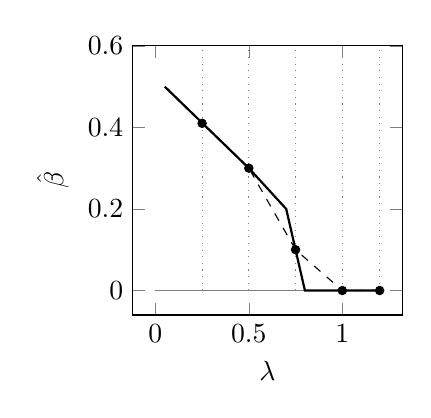
\begin{tikzpicture}
    \begin{axis}[
            ylabel = \(\hat\beta\),
            xlabel = \(\lambda\),
            % xmax = 1.4,
            % ymin = -0.1,
            ymax = 0.6,
            width = 5cm,
            height = 5cm
        ]
        \addplot[color = gray]
        coordinates {
                (0,0)
                (1.2,0)
            };
        \addplot[dotted, color = gray]
            coordinates {
                (1.2,0)
                (1.2,0.6)
            };
        \addplot[dotted, color = gray]
            coordinates {
                (1,0)
                (1,0.6)
            };
        \addplot[dotted, color = gray]
            coordinates {
                (0.75,0)
                (0.75,0.6)
            };
        \addplot[dotted, color = gray]
            coordinates {
                (0.5,0)
                (0.5,0.6)
            };
        \addplot[dotted, color = gray]
            coordinates {
                (0.25,0)
                (0.25,0.6)
            };
        \addplot[thick]
        coordinates {
                (1.2,0)
                (1,0)
                (0.8,0)
                (0.7, 0.2)
                (0.5, 0.3)
                (0.05, 0.5)
            };
        \addplot[mark=*, mark options = {style = solid, scale = 0.75}, solid, style = dashed]
        coordinates {
                (1.2,0)
                (1,0)
                (0.75, 0.1)
                (0.5, 0.3)
                (0.25, 0.41)
            };

        % \node [right] at (0.5,0) {\footnotesize\(\lambda_{k + 1}\)};
        % \node [right] at (0.8,0) {\footnotesize\(\lambda_{k}\)};
    \end{axis}
\end{tikzpicture}

      %   \caption{The exact path of a coefficient and the interpolated path
      %     based
      %     on the grid method as a dashed line.}
      % \end{figure}
    \end{column}
  \end{columns}
\end{frame}

\begin{frame}{Lasso Path Profiles}
  When and how predictors are activated along the lasso path varies.
  \begin{figure}
    \includegraphics{figures/grid-paths.pdf}
    \caption{The number of included predictors at each step along the path for
    the standard grid path for the lasso. The number of included predictors
  varies considerably from data set to data set.\label{fig:grid-paths}}
  \end{figure}
\end{frame}

\begin{frame}{The Adaptive Lasso Path}
  The gradient estimate from the Hessian screening rule can be used to predict
  at which \(\lambda\) values the predictors will enter the model. \medskip

  With the Adaptive Lasso Path, we use this information to find the next
  \(\lambda\) at which a desired number of predictors will enter the model
  \medskip

  This lets us decide the resolution of the lasso path arbitrarily.
  %   \begin{equation*}
  %   \hat\lambda_j =
  %   \begin{cases}
  %     \max
  %     \left\{
  %       \splitfrac{\frac{c(\lambda)_j - \lambda \nabla c(\lambda)_j}
  %         {1 - \nabla c(\lambda)_j},}{\frac{\lambda \nabla c(\lambda)_j -
  %           c(\lambda)_j}{1 + \nabla c(\lambda)_j}}
  %     \right\}
  %      & \text{if } \hat\beta(\lambda)_j = 0,    \\
  %     \frac{\hat\beta(\lambda)_j +
  %       \lambda}{\Big(H_\mathcal{A}^{-1}
  %       \sign\big(\hat\beta(\lambda_j)\big)\Big)_j}
  %      & \text{if } \hat\beta(\lambda)_j \neq 0.
  %   \end{cases}
  % \end{equation*}
\end{frame}

\begin{frame}{An Example}
  \begin{figure}
    \includegraphics{figures/case-study.pdf}
    \caption{The number of predictors entering the model at each step for
      either
      the adaptive path or the grid path.}
  \end{figure}
\end{frame}

\begin{frame}{}
  \begin{figure}
    \includegraphics[width=0.6\linewidth]{figures/max-error.pdf}
    \caption{Maximum error along the regularization path for the adaptive and
      grid methods. Scenario 1 is a high-dimensional setting and 2 a
      low-dimensional setup.}
  \end{figure}

\end{frame}

\begin{frame}{Discussion}
  \begin{itemize}
    \item The default grid heuristic is crude and sub-optimal in some cases.
    \item The adaptive lasso path adapts to the structure of the data and can be
      controlled by the user to tailor the resolution of the path.
    \item As \(n\) becomes smaller, the method converges towards a homotopy
      method.
  \end{itemize}
\end{frame}

\begin{frame}{Thank You!}
  Thank you for listening! Questions? Thoughts?
\end{frame}


\begin{frame}[allowframebreaks]{References}
  \bibliographytrue
  \printbibliography[heading=none]
\end{frame}

\end{document}
